Le note musicali si possono classificare nel seguente modo:
\begin{figure}[H]
	\centering
	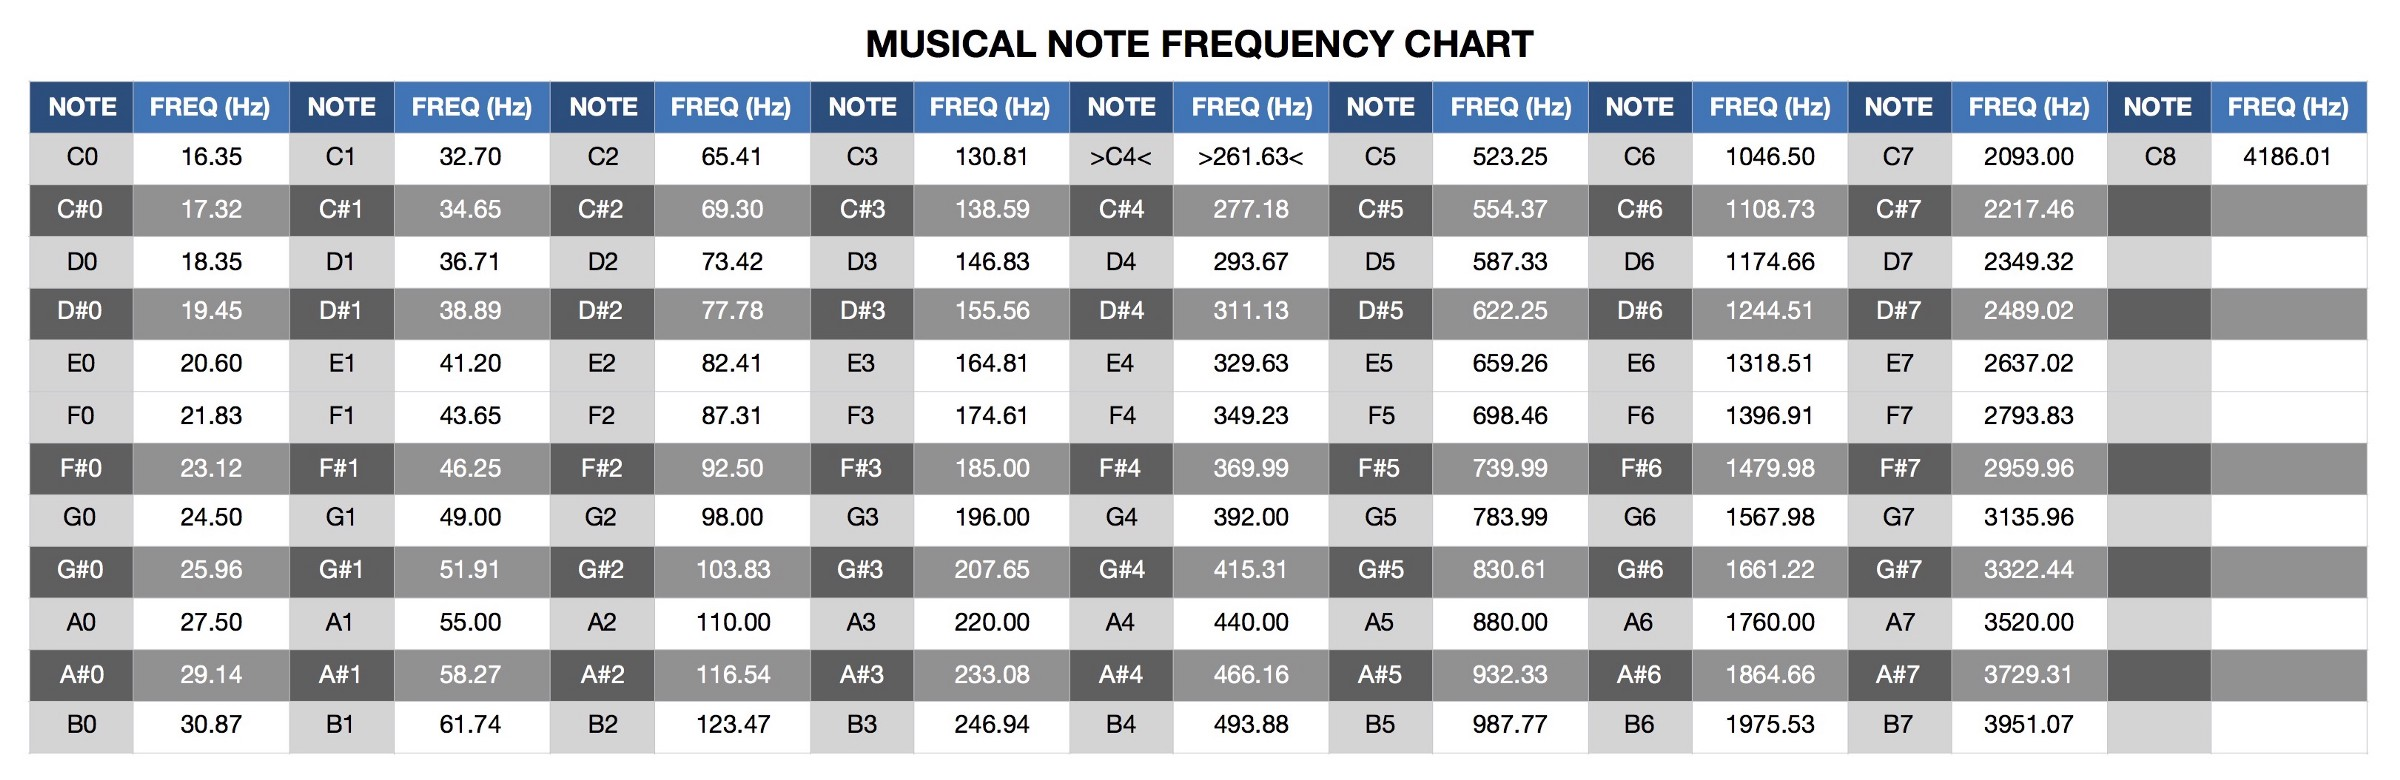
\includegraphics[scale=0.17]{./images/img4.jpg}
\end{figure}
\noindent La lettera a sinistra identifica la nota musicale mentre il numero a destra rappresenta la sua frequenza.\\
In musica, un'\textbf{ottava} è l'intervallo di otto note posizionate a frequenza diversa nella scala musicale. Le frequenze intermedie sono altre sei note. La frequenza tra una nota di un'ottava e la stessa nota di un'ottava successiva è doppia. Per esempio, il \textit{La} centrale (A4) ha frequenza di 440 Hz, il \textit{La} (A5) posto un'ottava sopra ha frequenza 880 Hz, quello un'ottava sotto (A3) ha frequenza 220 Hz.\\
Se si rappresentassero le prime sei ottave della nota \textit{Do} (C) potremmo vedere che la sua frequenza raddoppia ad ogni ottava.\\
\newline
I tasti che intercorrono fra gli estremi della stessa ottava (esempio \textit{Do} (C4) - \textit{Do} (C5)) sono dodici semitoni per cui la frequenza deve raddoppiare ogni dodici semitoni. Si può rappresentare quanto detto dalla seguente formula:
\vspace*{2ex}
\begin{center}
	\begin{math}
		F_{k}=440Hz \cdot 2^{k \over 12}
	\end{math}
\end{center}

Nel campo della musica viene utilizzata la trasformata a Q costante, a discapito della più nota trasformata di Fourier, proprio per la sua natura esponenziale. Inoltre, l'accuratezza della trasformata a Q costante è analoga alla scala logaritmica e imita l'orecchio umano, avendo una risoluzione di frequenza più alta a quelle più basse e una risoluzione più bassa alle frequenze più alte. Infatti, dal seguente grafico si può notare la natura esponenziale della funzione:
\vspace*{2ex}
\begin{center}
	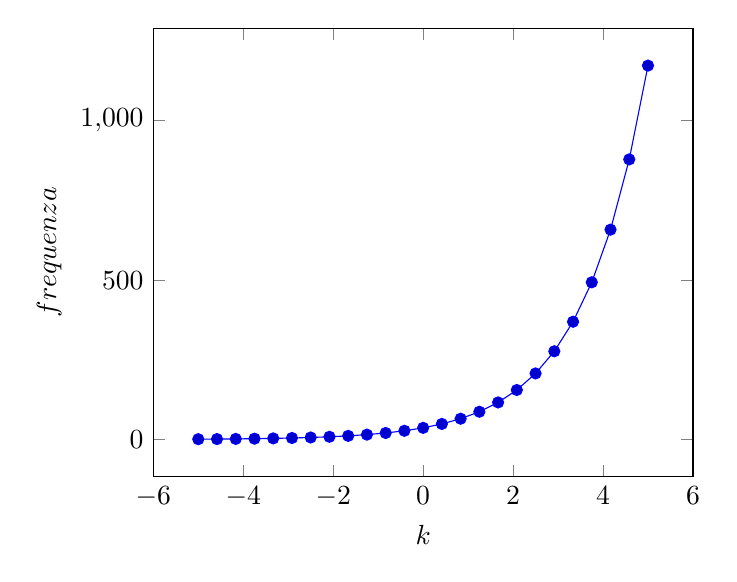
\begin{tikzpicture}
	\begin{axis}[ 
		xlabel=$k$,
		ylabel={$frequenza$}
		] 
		\addplot {440*2^x/12}; 
	\end{axis}
\end{tikzpicture}
\end{center}